\begin{center}
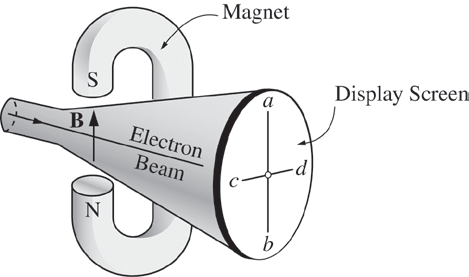
\includegraphics[scale=0.5]{images/img-008-021.png}
\end{center}

% Multiple Choice Question 29
\begin{questions}\setcounter{question}{28}\question
A horizontal electron beam in an oscilloscope is aimed at the center of the display screen, as shown in the diagram above. A C-shaped magnet is placed around the oscilloscope, producing a vertical magnetic field $\mathbf{B}$, which is perpendicular to the beam. Which way, if any, will the beam be deflected by the magnetic field?

\begin{choices}
\choice Toward point $a$
\choice Toward point $b$
\choice Toward point $c$
\choice Toward point $d$
\choice The beam will not be deflected.
\end{choices}\end{questions}

